\clearpage

\section{方法}
\subsection{使用器具}
今回の実験で使用した器具を\wtab{kigu}に示す.
\begin{table}[h]
\centering
\caption{使用器具}
\label{tab:kigu}
\begin{tabular}{cccc}
\hline
器具名     & 製造会社                 & 型番                    & シリアルナンバー        \\ \hline
電力計     & 横河計測                 & MODEL 2041            & L98-000218      \\
電流計     & 横河計測                 & TYPE 2013             & L94-004860      \\
電圧計     & 横河計測                 & TYPE 2052             & B-5033.62.14/14 \\
スライダック  & 東京理工舎                & RIKO-SLIDETRANS RSA-2 & S57-5.1/15      \\
オシロスコープ & Agilent Technologies & DSO1022A              & CN53504828      \\
トランス    & 菅野電機研究所(株)           & MODEL SP-121          & No.2            \\ \hline
\end{tabular}
\end{table}
\subsection{実験手順}
\begin{enumerate}[(a)]
	\item 励磁電流の観測
	\begin{enumerate}[i)]
	\item \wfig{circ}のように回路を構築した.
	\begin{figure}[h]
	\centering
	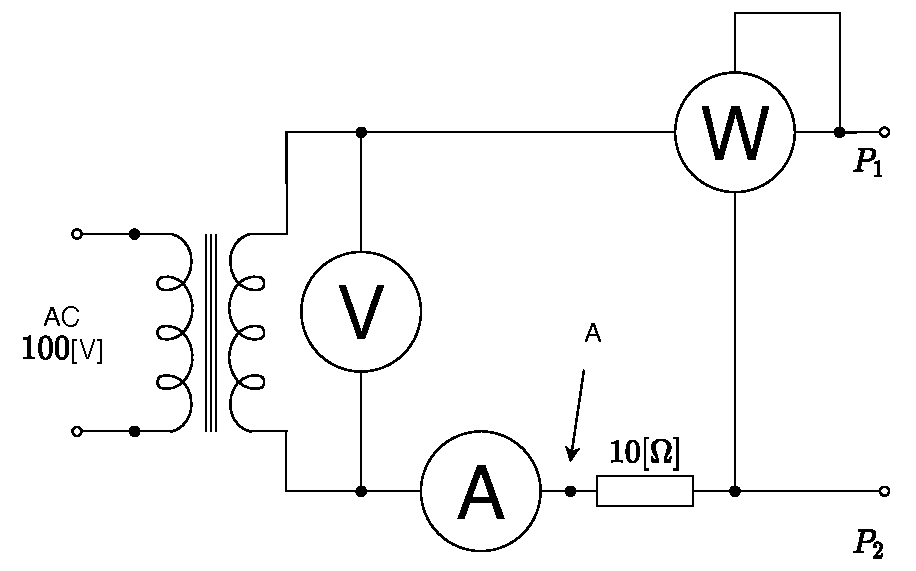
\includegraphics[scale=1]{./fig/circ.pdf}
	\caption{測定回路}
	\label{fig:circ}
	\end{figure}
	\item オシロスコープの水平感度は$5\,\rm{ms/DIV}$に設定.
	\item オシロスコープのch1プローブのGNDを同図の$P_{2}$へ,プローブの先をA点に接続し,ch2のプローブのGNDを$P_{2}$へ,プローブの先を$P_{1}$に接続.
	\item ch2の信号を反転させるように設定を変更.\footnote{INVスイッチを押す}
	\item ch1の垂直感度を$0.5\,\rm{V/DIV}$に,ch2垂直感度を$50\,\rm{V/DIV}$に設定.
	\item 入力電圧を$75\,\rm{V}\sim 100\,\rm{V}$まで$5\,\rm{V}$刻みで変化させ,それぞれの場合においての電流と電力を計測した.
	\item 位相差$\theta$はExcelで\weq{siki}を算出して求めた.
	\begin{equation}
		\theta=\cos^{-1}\frac{P_{0}}{Vi_{0}}
		\label{eq:siki}
	\end{equation}
	\item $80\,\rm{V}$と$100\,\rm{V}$の場合においては入力電圧波形及び励磁電流の波形を保存した.
\end{enumerate}
\item ヒステリシス曲線の測定
\begin{enumerate}[i)]
	\item \wfig{circ}の$P_{1}$に\wfig{ad}の$S_{1}$を\wfig{circ}の$P_{2}$に\wfig{ad}の$S_{2}$を接続.
	\begin{figure}[h]
	\centering
	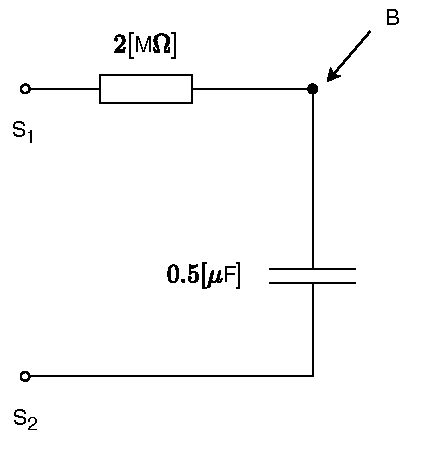
\includegraphics[scale=1]{./fig/ad.pdf}
	\caption{積分回路}
	\label{fig:ad}
	\end{figure}
	\item ch1の垂直感度を$0.5\,\rm{V/DIV}$とし,ch2の垂直感度は$20\,\rm{mV/DIV}$に設定.
	\item ch1プローブのGNDを\wfig{circ}の$P_{2}$へ,プローブの先をA点に接続し,ch2のプローブのGNDを\wfig{ad}のB点へ,プローブの先を$S_{2}$に接続.
	\item ch2の信号の反転をしたままの状態にした.
	\item 表示をX-Y 表示に変更.
	\item 入力電圧が$80\,\rm{V}$, $100\,\rm{V}$のそれぞれの場合においての波形を記録した.
\end{enumerate}
\end{enumerate}
